\documentclass[12pt,leqno]{article}

\usepackage[english]{babel}
\usepackage{amsmath}
\usepackage{amssymb}
\usepackage{amsthm}
\usepackage{graphicx}


\title{pestim - an R package to estimate population counts from aggregated mobile phone data}
\author{David Salgado \footnote{Deptartment of Methodology and Development of Statistical Production. Statistics Spain (INE)} and 
 who else to add as author??}
\date{}


\newtheorem{lemma}{Lemma}
\newcommand{\appropto}{\mathrel{\vcenter{
  \offinterlineskip\halign{\hfil$##$\cr
    \propto\cr\noalign{\kern2pt}\sim\cr\noalign{\kern-2pt}}}}}


\begin{document}
\maketitle

\begin{abstract}
Two of the most used measures for inequality in the study of income and
wealth distributions are the Gini ($G$) and Theil ($T$) indices. 
While there is a vast literature on the bounds of these two measures given
partial information about the income distribution, 
the relationship between them has been less studied.
In this paper we investigate whether there is a lower and upper bound for 
the $T$ index at a given value of the $G$ index, 
for both continuous and discrete distributions. We derive a theoretical 
lower bound for $T$ at given $G$, and show that
there is no corresponding upper bound, and $T$ can be made as large as desired 
by choosing an appropriate form of the Lorenz curve. We illustrate the bound
for several parametric models of income distribution and Lorenz curves 
frequently used in the income inequality literature.

 
	
\end{abstract}


\section{Introduction}

{\textit{pestim}} R package implements a hierarchical model to estimate the population counts of different territorial cells combining the information from aggregated 
mobile phone data and a population register or survey data, both at a given time instant and along a 
sequence of time periods. The theoretical model implemented by the {\textit{pestim}} R package
follows the ecological sampling techniques to estimate population counts (see e.g. \cite{ManNacAlb15a} and 
\cite {RoyDor08a} which are based on a bayesian approach. The complete methodology is described in \cite{methdology}.

The inference of the population counts from mobile phone data and official data is acheived in a two step process:
\begin{itemize}
\item{at a given time instant $t{0}$ both mobile phone and 
official data are used to infer the population counts in each territorial cell;}
\item{at later moments, $t_{1}, t_{2}, \...$ the transition probabilities are inferred from mobile phone data and are used to estimate the spatial and time evolution of the population.}
\end{itemize}




\section{The hierarchical model}\label{model}

In this section we will give a short description of the theoretical model underlaying the {\textit{pestim}} R package for estimation of the population counts at a given time moment.

A first input in the model is $\mathbf{N}^{\textrm{MNO}}=(N_{1}^{\textrm{MNO}}, \dots, N_{I}^{\textrm{MNO}})^{T}$ which represents the population counts reported by the mobile network operator in each territorial cell $i\in\mathcal{I}=\{1,\dots,I\}$ (i.e. the aggregated mobile phone data).  The second input of the model is the official population counts in each territorial cell denoted by 
$\mathbf{N}^{\textrm{REG}}=(N_{1}^{\textrm{REG}}, \dots, N_{I}^{\textrm{REG}})^{T}$. These official population counts could come from administrative data sources or from statistical surveys.
 {\textit{pestim}} implements a function to estimate the actual population counts $\mathbf{N}=(N_{1}, \dots, N_{I})^{T}$ combining both data sources. It also compute the posterior probability distribution 
$\mathbb{P}\left(\mathbf{N}|\mathbf{N}^{\textrm{MNO}};\mathbf{N}^{\textrm{REG}}\right)$ 
that can be used to assess the uncertainty in the output estimates.
This process can be represented schematically as follows.

\begin{figure}[htbp]
\centering
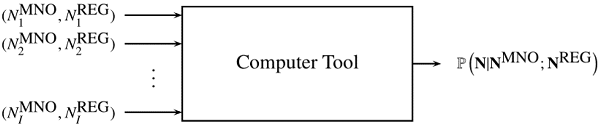
\includegraphics{Tool.png}
\caption{\label{Tool} A diagram for the process of estimating population counts using mobile phone and official population data.}
\end{figure}




\begin{thebibliography}{99}

\bibitem{ManNacAlb15a}
~Manly, B.F.J., ~ Navarro Alberto, J.A., Introduction to ecological sampling,
CRC Press, 2015.

\bibitem{RoyDor08a}
~Royle, J.A., Dorazio, R.M., Hierarchical modeling and inference in ecology,
Academic Press, 2008.

\bibitem{BDA3}
~Gelman, A., ~Carlin, J.B., ~Stern, H.S., ~Dunson, D.B., ~Vehtari, A., ~Rubin, D.B., Bayesian Data Analysis (3rd ed), CRC Press, 2013

\bibitem{FlaSed95a}
~Flajolet, P., ~Sedgewick, R.,  Mellin transforms and asymptotics; Finite differences and Rice's integrals,
in  Theoretical Computer Science 144, pp. 101-124, 1995.


\bibitem{GraKnuPat96a}
Graham, R.L., ~Knuth, D.E., ~Patashnik, O., Concrete Mathematics (2nd ed.), 
Addison-Wesley, 1996.


\bibitem{Joh02a}
~Johnson, W.P., The curious history of Faà di Bruno's formula, in 
American Mathematical Monthly 109, pp. 217-234, March, 2002.


\bibitem{BroChu03a}
~Brown, J.W., ~Churchill, R.V., Complex variables and applications (7th ed.), 2003.

\bibitem{GraRyz07a}
~Gradshteyn, I.S., ~Ryzhik, I.M., Tables of Integrals, Series, and Products (7th ed.),
2007.

\bibitem{Dev86a}
~Devroye, L., Non-uniform random variable generation, Springer, 1986.

\bibitem{Q2016}
~De Meersman, F., ~Seynaeve, G., ~Debusschere, M., ~Lusyne, P., ~Dewitte, P., 
~Baeyens, Y., ~Wirthmann, A., ~Demunter, C., ~Reis, F., ~Reuter, H.I.,
Assessing the Quality of Mobile Phone Data as a Source of Statistics,
presented at Q2016 Conference, June, 2016.

\bibitem{WP5Del11}
~ESSnet on Big Data WP5, Current status of access to mobile phone data in the ESS, 2017.
 
\end{thebibliography}


\end{document}